\documentclass{ximera}

%\usepackage{todonotes}

\newcommand{\todo}{}

\usepackage{esint} % for \oiint
\ifxake%%https://math.meta.stackexchange.com/questions/9973/how-do-you-render-a-closed-surface-double-integral
\renewcommand{\oiint}{{\large\bigcirc}\kern-1.56em\iint}
\fi


\graphicspath{
  {./}
  {ximeraTutorial/}
  {basicPhilosophy/}
  {functionsOfSeveralVariables/}
  {normalVectors/}
  {lagrangeMultipliers/}
  {vectorFields/}
  {greensTheorem/}
  {shapeOfThingsToCome/}
  {dotProducts/}
  {partialDerivativesAndTheGradientVector/}
  {../productAndQuotientRules/exercises/}
  {../normalVectors/exercisesParametricPlots/}
  {../continuityOfFunctionsOfSeveralVariables/exercises/}
  {../partialDerivativesAndTheGradientVector/exercises/}
  {../directionalDerivativeAndChainRule/exercises/}
  {../commonCoordinates/exercisesCylindricalCoordinates/}
  {../commonCoordinates/exercisesSphericalCoordinates/}
  {../greensTheorem/exercisesCurlAndLineIntegrals/}
  {../greensTheorem/exercisesDivergenceAndLineIntegrals/}
  {../shapeOfThingsToCome/exercisesDivergenceTheorem/}
  {../greensTheorem/}
  {../shapeOfThingsToCome/}
  {../separableDifferentialEquations/exercises/}
  {vectorFields/}
}

\newcommand{\mooculus}{\textsf{\textbf{MOOC}\textnormal{\textsf{ULUS}}}}

\usepackage{tkz-euclide}
\usepackage{tikz}
\usepackage{tikz-cd}
\usetikzlibrary{arrows}
\tikzset{>=stealth,commutative diagrams/.cd,
  arrow style=tikz,diagrams={>=stealth}} %% cool arrow head
\tikzset{shorten <>/.style={ shorten >=#1, shorten <=#1 } } %% allows shorter vectors

\usetikzlibrary{backgrounds} %% for boxes around graphs
\usetikzlibrary{shapes,positioning}  %% Clouds and stars
\usetikzlibrary{matrix} %% for matrix
\usepgfplotslibrary{polar} %% for polar plots
\usepgfplotslibrary{fillbetween} %% to shade area between curves in TikZ
%\usetkzobj{all}
\usepackage[makeroom]{cancel} %% for strike outs
%\usepackage{mathtools} %% for pretty underbrace % Breaks Ximera
%\usepackage{multicol}
\usepackage{pgffor} %% required for integral for loops



%% http://tex.stackexchange.com/questions/66490/drawing-a-tikz-arc-specifying-the-center
%% Draws beach ball
\tikzset{pics/carc/.style args={#1:#2:#3}{code={\draw[pic actions] (#1:#3) arc(#1:#2:#3);}}}



\usepackage{array}
\setlength{\extrarowheight}{+.1cm}
\newdimen\digitwidth
\settowidth\digitwidth{9}
\def\divrule#1#2{
\noalign{\moveright#1\digitwidth
\vbox{\hrule width#2\digitwidth}}}




% \newcommand{\RR}{\mathbb R}
% \newcommand{\R}{\mathbb R}
% \newcommand{\N}{\mathbb N}
% \newcommand{\Z}{\mathbb Z}

\newcommand{\sagemath}{\textsf{SageMath}}


%\renewcommand{\d}{\,d\!}
%\renewcommand{\d}{\mathop{}\!d}
%\newcommand{\dd}[2][]{\frac{\d #1}{\d #2}}
%\newcommand{\pp}[2][]{\frac{\partial #1}{\partial #2}}
% \renewcommand{\l}{\ell}
%\newcommand{\ddx}{\frac{d}{\d x}}

% \newcommand{\zeroOverZero}{\ensuremath{\boldsymbol{\tfrac{0}{0}}}}
%\newcommand{\inftyOverInfty}{\ensuremath{\boldsymbol{\tfrac{\infty}{\infty}}}}
%\newcommand{\zeroOverInfty}{\ensuremath{\boldsymbol{\tfrac{0}{\infty}}}}
%\newcommand{\zeroTimesInfty}{\ensuremath{\small\boldsymbol{0\cdot \infty}}}
%\newcommand{\inftyMinusInfty}{\ensuremath{\small\boldsymbol{\infty - \infty}}}
%\newcommand{\oneToInfty}{\ensuremath{\boldsymbol{1^\infty}}}
%\newcommand{\zeroToZero}{\ensuremath{\boldsymbol{0^0}}}
%\newcommand{\inftyToZero}{\ensuremath{\boldsymbol{\infty^0}}}



% \newcommand{\numOverZero}{\ensuremath{\boldsymbol{\tfrac{\#}{0}}}}
% \newcommand{\dfn}{\textbf}
% \newcommand{\unit}{\,\mathrm}
% \newcommand{\unit}{\mathop{}\!\mathrm}
% \newcommand{\eval}[1]{\bigg[ #1 \bigg]}
% \newcommand{\seq}[1]{\left( #1 \right)}
% \renewcommand{\epsilon}{\varepsilon}
% \renewcommand{\phi}{\varphi}


% \renewcommand{\iff}{\Leftrightarrow}

% \DeclareMathOperator{\arccot}{arccot}
% \DeclareMathOperator{\arcsec}{arcsec}
% \DeclareMathOperator{\arccsc}{arccsc}
% \DeclareMathOperator{\si}{Si}
% \DeclareMathOperator{\scal}{scal}
% \DeclareMathOperator{\sign}{sign}


%% \newcommand{\tightoverset}[2]{% for arrow vec
%%   \mathop{#2}\limits^{\vbox to -.5ex{\kern-0.75ex\hbox{$#1$}\vss}}}
% \newcommand{\arrowvec}[1]{{\overset{\rightharpoonup}{#1}}}
% \renewcommand{\vec}[1]{\arrowvec{\mathbf{#1}}}
% \renewcommand{\vec}[1]{{\overset{\boldsymbol{\rightharpoonup}}{\mathbf{#1}}}}

% \newcommand{\point}[1]{\left(#1\right)} %this allows \vector{ to be changed to \vector{ with a quick find and replace
% \newcommand{\pt}[1]{\mathbf{#1}} %this allows \vec{ to be changed to \vec{ with a quick find and replace
% \newcommand{\Lim}[2]{\lim_{\point{#1} \to \point{#2}}} %Bart, I changed this to point since I want to use it.  It runs through both of the exercise and exerciseE files in limits section, which is why it was in each document to start with.

% \DeclareMathOperator{\proj}{\mathbf{proj}}
% \newcommand{\veci}{{\boldsymbol{\hat{\imath}}}}
% \newcommand{\vecj}{{\boldsymbol{\hat{\jmath}}}}
% \newcommand{\veck}{{\boldsymbol{\hat{k}}}}
% \newcommand{\vecl}{\vec{\boldsymbol{\l}}}
% \newcommand{\uvec}[1]{\mathbf{\hat{#1}}}
% \newcommand{\utan}{\mathbf{\hat{t}}}
% \newcommand{\unormal}{\mathbf{\hat{n}}}
% \newcommand{\ubinormal}{\mathbf{\hat{b}}}

% \newcommand{\dotp}{\bullet}
% \newcommand{\cross}{\boldsymbol\times}
% \newcommand{\grad}{\boldsymbol\nabla}
% \newcommand{\divergence}{\grad\dotp}
% \newcommand{\curl}{\grad\cross}
%\DeclareMathOperator{\divergence}{divergence}
%\DeclareMathOperator{\curl}[1]{\grad\cross #1}
% \newcommand{\lto}{\mathop{\longrightarrow\,}\limits}

% \renewcommand{\bar}{\overline}

\colorlet{textColor}{black}
\colorlet{background}{white}
\colorlet{penColor}{blue!50!black} % Color of a curve in a plot
\colorlet{penColor2}{red!50!black}% Color of a curve in a plot
\colorlet{penColor3}{red!50!blue} % Color of a curve in a plot
\colorlet{penColor4}{green!50!black} % Color of a curve in a plot
\colorlet{penColor5}{orange!80!black} % Color of a curve in a plot
\colorlet{penColor6}{yellow!70!black} % Color of a curve in a plot
\colorlet{fill1}{penColor!20} % Color of fill in a plot
\colorlet{fill2}{penColor2!20} % Color of fill in a plot
\colorlet{fillp}{fill1} % Color of positive area
\colorlet{filln}{penColor2!20} % Color of negative area
\colorlet{fill3}{penColor3!20} % Fill
\colorlet{fill4}{penColor4!20} % Fill
\colorlet{fill5}{penColor5!20} % Fill
\colorlet{gridColor}{gray!50} % Color of grid in a plot

\newcommand{\surfaceColor}{violet}
\newcommand{\surfaceColorTwo}{redyellow}
\newcommand{\sliceColor}{greenyellow}




\pgfmathdeclarefunction{gauss}{2}{% gives gaussian
  \pgfmathparse{1/(#2*sqrt(2*pi))*exp(-((x-#1)^2)/(2*#2^2))}%
}


%%%%%%%%%%%%%
%% Vectors
%%%%%%%%%%%%%

%% Simple horiz vectors
\renewcommand{\vector}[1]{\left\langle #1\right\rangle}


%% %% Complex Horiz Vectors with angle brackets
%% \makeatletter
%% \renewcommand{\vector}[2][ , ]{\left\langle%
%%   \def\nextitem{\def\nextitem{#1}}%
%%   \@for \el:=#2\do{\nextitem\el}\right\rangle%
%% }
%% \makeatother

%% %% Vertical Vectors
%% \def\vector#1{\begin{bmatrix}\vecListA#1,,\end{bmatrix}}
%% \def\vecListA#1,{\if,#1,\else #1\cr \expandafter \vecListA \fi}

%%%%%%%%%%%%%
%% End of vectors
%%%%%%%%%%%%%

%\newcommand{\fullwidth}{}
%\newcommand{\normalwidth}{}



%% makes a snazzy t-chart for evaluating functions
%\newenvironment{tchart}{\rowcolors{2}{}{background!90!textColor}\array}{\endarray}

%%This is to help with formatting on future title pages.
\newenvironment{sectionOutcomes}{}{}



%% Flowchart stuff
%\tikzstyle{startstop} = [rectangle, rounded corners, minimum width=3cm, minimum height=1cm,text centered, draw=black]
%\tikzstyle{question} = [rectangle, minimum width=3cm, minimum height=1cm, text centered, draw=black]
%\tikzstyle{decision} = [trapezium, trapezium left angle=70, trapezium right angle=110, minimum width=3cm, minimum height=1cm, text centered, draw=black]
%\tikzstyle{question} = [rectangle, rounded corners, minimum width=3cm, minimum height=1cm,text centered, draw=black]
%\tikzstyle{process} = [rectangle, minimum width=3cm, minimum height=1cm, text centered, draw=black]
%\tikzstyle{decision} = [trapezium, trapezium left angle=70, trapezium right angle=110, minimum width=3cm, minimum height=1cm, text centered, draw=black]


\title{Describe Everything}

\begin{document}

\begin{abstract}
features
\end{abstract}
\maketitle





\begin{example}  Complete Analysis


Completely analyze   

\[   B(f) = \frac{(f+3)(f-1)}{(f+5)(f-2)^2}        \]


\begin{explanation}



The natural domain is all real numbers except $-5$ and $2$, which make the denominator equal to $0$. These are singularities of $B$.  Otherwise, $B$ is continuous.  There are no discontinuities.

Domain = $(-\infty, -5) \cup (-5, 2) \cup (2, \infty)$

The graph will help us with the range, so we'll wait on that.

$B$ has zeros at $\answer{-3}$ and $\answer{1}$.  These make the numerator equal to $0$. These are represented on the graph with $(-3,0)$ and $(1,0)$

The graph will have vertical asymptotes $f=-5$ and $f=-2$.  $B$ will change sign over $f=-5$, since the multiplicity is \wordChoice{\choice[correct]{odd} \choice{even}} .  $B$ will not change sign over $f=2$, since the multiplicity is \wordChoice{\choice{odd} \choice[correct]{even}}.

$B$ is a rational function and the degree of the denominator is \wordChoice{\choice[correct]{greater than} \choice{less than}} the degree of the numerator. Therefore, 


\[ \lim_{f \to -\infty} B(f) = \answer{0}   \, \text{ and }  \,  \lim_{f \to \infty} B(f) = \answer{0}    \]


The graph has a horizontal asymptote at $y=\answer{0}$. \\

From this, we can sketch a graph of $y = B(f)$. \\






\begin{image}
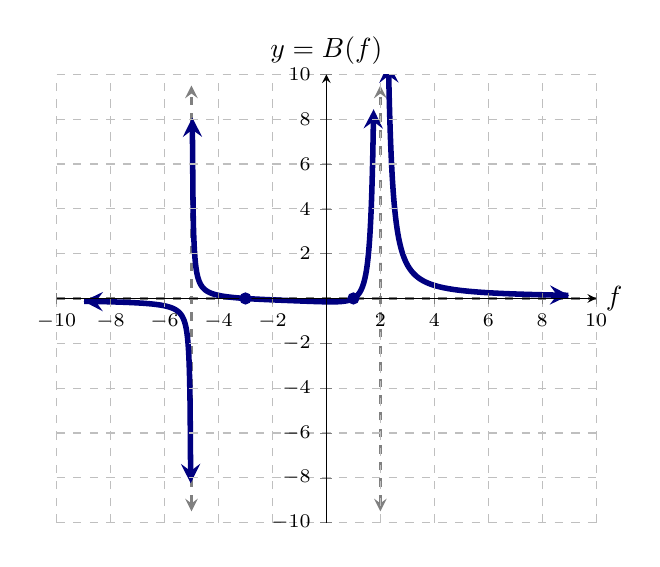
\begin{tikzpicture}
  \begin{axis}[
            domain=-10:10, ymax=10, xmax=10, ymin=-10, xmin=-10,
            axis lines =center, xlabel=$f$, ylabel={$y=B(f)$}, grid = major, grid style={dashed},
            ytick={-10,-8,-6,-4,-2,2,4,6,8,10},
            xtick={-10,-8,-6,-4,-2,2,4,6,8,10},
            yticklabels={$-10$,$-8$,$-6$,$-4$,$-2$,$2$,$4$,$6$,$8$,$10$}, 
            xticklabels={$-10$,$-8$,$-6$,$-4$,$-2$,$2$,$4$,$6$,$8$,$10$},
            ticklabel style={font=\scriptsize},
            every axis y label/.style={at=(current axis.above origin),anchor=south},
            every axis x label/.style={at=(current axis.right of origin),anchor=west},
            axis on top
          ]
          

          \addplot [line width=1, gray, dashed, domain=(-9.5:9.5),<->] ({-5},{x});
          \addplot [line width=1, gray, dashed, domain=(-9.5:9.5),<->] ({2},{x});
          \addplot [line width=1, gray, dashed, domain=(-10:10)] {0};



          \addplot [line width=2, penColor, smooth,samples=200,domain=(-9:-5.03),<->] {((x+3)*(x-1))/((x+5)*(x-2)^2)};
          \addplot [line width=2, penColor, smooth,samples=200,domain=(-4.97:1.75),<->] {((x+3)*(x-1))/((x+5)*(x-2)^2)};
          \addplot [line width=2, penColor, smooth,samples=200,domain=(2.3:9),<->] {((x+3)*(x-1))/((x+5)*(x-2)^2)};

          \addplot[color=penColor,fill=penColor,only marks,mark=*] coordinates{(-3,0)};
          \addplot[color=penColor,fill=penColor,only marks,mark=*] coordinates{(1,0)};


           

  \end{axis}
\end{tikzpicture}
\end{image}


Both zeros have odd multiplicity, therefore the graph must go below the $f$-axis between them.  There must be a local minimum. From the graph we can estimate that the critical number is approximately $0.5$. $B(0.5) = \frac{14}{99} \approx -0.1414$ is a local minimum. With some Calculus tools, we may be able to get an exact value.


$B$ has no global maximum or minimum.

$B$ has no local maximum.


\begin{itemize}
\item $B$ decreases on $(-\infty, -5)$.
\item $B$ decreases on $(-5, 0.5)$.
\item $B$ increases on $(0.5, 2)$.
\item $B$ decreases on $(2, \infty)$.
\end{itemize}



The graph makes it evident that the range is all real numbers.






\begin{question}

$B(t)$ is decreasing on $(-\infty, -5)$ and $B(t)$ is decreasing on $(-5, 0.5)$.  Therefore, $B(t)$ is decreasing on $(-\infty, -5) \cup (-5, 0.5)$


\begin{multipleChoice}
\choice {True}
\choice [correct] {False}
\end{multipleChoice}
\end{question}

\end{explanation}

\end{example}








With some graphing tools, we can get a better approximation of the critical number.




\begin{center}
\desmos{sumsbfeafr}{400}{300}
\end{center}



The critical number is approximately $0.181$ and the local minimum value of $B$ is approximately $-1.152$.









\begin{example} Analyze


Completely analyze $K(w) = w \sqrt{9-w}$.


\begin{explanation}



The domain is restricted by the square root to be $\left( -\infty, \answer{9} \right]$.


The formula is a product, therefore the zeros come from each factor.

The factor of $w$ gives a zero of $\answer{0}$.

The factor of $\sqrt{9-w}$ gives a zero of $\answer{9}$.


Since $\sqrt{9-w}$ is always nonnegative, the sign of $K$ is the same as the sign of $w$.

\begin{itemize}
\item $K$ is negative on $\left( \answer{-\infty},\answer{0} \right)$
\item $K$ is positive on $\left( \answer{0}, \answer{\infty} \right)$
\end{itemize}




From this, we can sketch a graph of $y = K(w)$. \\






\begin{image}
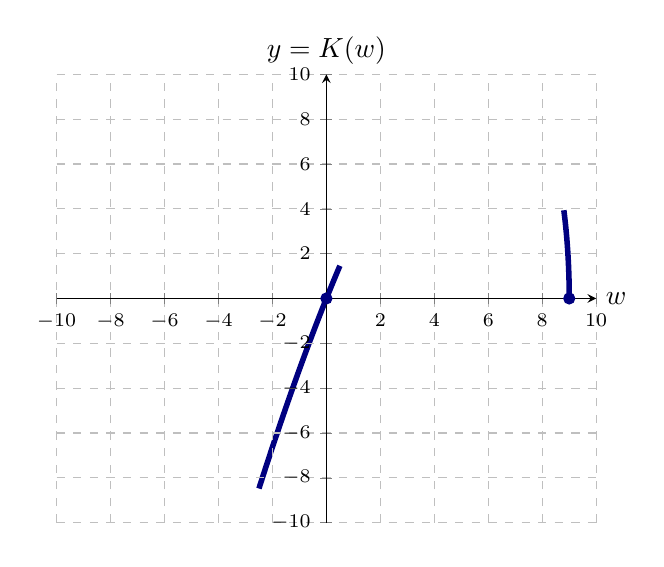
\begin{tikzpicture}
  \begin{axis}[
            domain=-10:10, ymax=10, xmax=10, ymin=-10, xmin=-10,
            axis lines =center, xlabel=$w$, ylabel={$y=K(w)$}, grid = major, grid style={dashed},
            ytick={-10,-8,-6,-4,-2,2,4,6,8,10},
            xtick={-10,-8,-6,-4,-2,2,4,6,8,10},
            yticklabels={$-10$,$-8$,$-6$,$-4$,$-2$,$2$,$4$,$6$,$8$,$10$}, 
            xticklabels={$-10$,$-8$,$-6$,$-4$,$-2$,$2$,$4$,$6$,$8$,$10$},
            ticklabel style={font=\scriptsize},
            every axis y label/.style={at=(current axis.above origin),anchor=south},
            every axis x label/.style={at=(current axis.right of origin),anchor=west},
            axis on top
          ]


          \addplot [line width=2, penColor, smooth,samples=200,domain=(-2.5:0.5)] {x * sqrt(9-x)};
          \addplot [line width=2, penColor, smooth,samples=200,domain=(8.8:9)] {x * sqrt(9-x)};


          \addplot[color=penColor,fill=penColor,only marks,mark=*] coordinates{(0,0)};
          \addplot[color=penColor,fill=penColor,only marks,mark=*] coordinates{(9,0)};


           

  \end{axis}
\end{tikzpicture}
\end{image}


Our sketch suggest a global maximum between $0$ and $9$.


If we had the derivative, then we could identify this critical number exactly. Currently, we'll need a graph to approximate values.




\begin{center}
\desmos{zbhmb5usvv}{400}{300}
\end{center}





\begin{itemize}
\item $K$ has a local and global maximum of $10.39$ at $6$.
\item $K$ has a local minimum of $0$ at $9$.
\item $K$ has no global minimum.
\end{itemize}




\begin{itemize}
\item $K$ is increasing on $(-\infty, 6]$.
\item $K$ is decreasing on $[6, 9]$.
\end{itemize}


Finally, the range is approximately $(-\infty, 10.39]$. \\


The graph has no vertical asymptotes, $\lim\limits_{w \to -\infty} K(w) = -\infty.$

\end{explanation}

\end{example}



We do have alternatives to the derivative for some types of functions. \\







\begin{procedure} Critical Number


Earlier, we saw an algebraic method of identifying the critical number in the previous example.


We think there is a hump in the graph of $K$ and at the highest point, $(A, A\sqrt{9-A})$, the tangent line would be horizontal.



\begin{image}
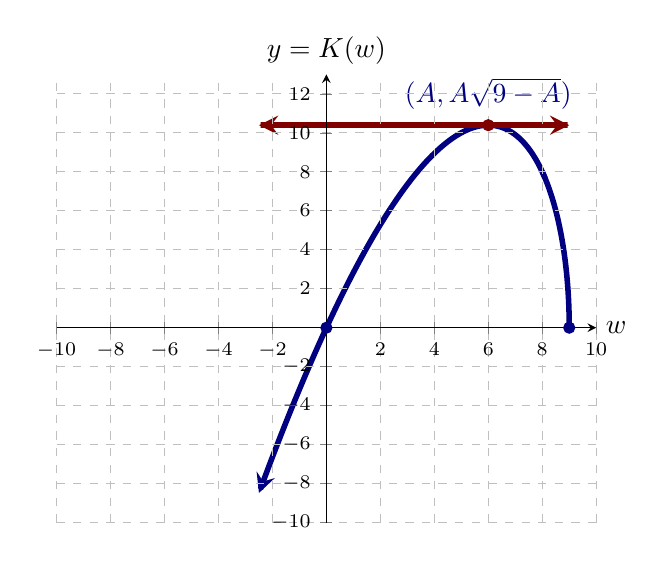
\begin{tikzpicture}
  \begin{axis}[
            domain=-10:10, ymax=13, xmax=10, ymin=-10, xmin=-10,
            axis lines =center, xlabel=$w$, ylabel={$y=K(w)$}, grid = major, grid style={dashed},
            ytick={-10,-8,-6,-4,-2,2,4,6,8,10,12},
            xtick={-10,-8,-6,-4,-2,2,4,6,8,10},
            yticklabels={$-10$,$-8$,$-6$,$-4$,$-2$,$2$,$4$,$6$,$8$,$10$,$12$}, 
            xticklabels={$-10$,$-8$,$-6$,$-4$,$-2$,$2$,$4$,$6$,$8$,$10$},
            ticklabel style={font=\scriptsize},
            every axis y label/.style={at=(current axis.above origin),anchor=south},
            every axis x label/.style={at=(current axis.right of origin),anchor=west},
            axis on top
          ]


          \addplot [line width=2, penColor, smooth,samples=200,domain=(-2.5:8.1),<-] {x * sqrt(9-x)};
          \addplot [line width=2, penColor, smooth,samples=300,domain=(8:9)] {x * sqrt(9-x)};
          \addplot [line width=2, penColor2, smooth,samples=200,domain=(-2.5:9),<->] {10.39};
         


          \addplot[color=penColor,fill=penColor,only marks,mark=*] coordinates{(0,0)};
          \addplot[color=penColor,fill=penColor,only marks,mark=*] coordinates{(9,0)};
          \addplot[color=penColor2,fill=penColor2,only marks,mark=*] coordinates{(6,10.39)};


          \node at (axis cs:6,12) [penColor] {$(A, A\sqrt{9-A})$};


           

  \end{axis}
\end{tikzpicture}
\end{image}


Now, create a new function called $F$.

\[
F(x) = K(x) - K(A) = K(x) - A\sqrt{9-A}
\]


As we saw earlier, since we have a tangent line, the difference of the original function and the linear function has a double root at $A$.  $x-A$ divides evenly into $F$.  And, the resulting function then also has $A$ as a root.  

First, factor out $x-A$ from $F$.


\[
x\sqrt{9-x} - A\sqrt{9-A} = \frac{x\sqrt{9-x} - A\sqrt{9-A}}{1} \cdot \frac{x\sqrt{9-x} + A\sqrt{9-A}}{\answer{x\sqrt{9-x} + A\sqrt{9-A}}}
\]

\[
= \frac{x^2 (9-x) - A^2 (9-A)}{x\sqrt{9-x} + A\sqrt{9-A}} = \frac{9x^2 - x^3 - 9A^2 + A^3}{x\sqrt{9-x} + A\sqrt{9-A}}
\]


\[
= \frac{9(x^2-A^2) - (x^3 - A^3)}{x\sqrt{9-x} + A\sqrt{9-A}} = \frac{(x-A)(9(x+A)-(x^2 + xA + A^2))}{x\sqrt{9-x} + A\sqrt{9-A}}
\]


$x-A$ divides into this evenly leaving

\[
\frac{9(x+A)-(x^2 + xA + A^2)}{x\sqrt{9-x} + A\sqrt{9-A}}
\]

$A$ is a root of this, which means $A$ is a root of the numerator.


\[
9(A+A)-(A^2 + A^2 + A^2) = 0
\]

\[
18A - 3A^2 = 0
\]

\[
3A \left(\answer{6-A} \right) = 0
\]


The zero we are looking for is $6$.
The critical number is $6$ and $K(6) = 6 \sqrt{3}$.


\end{procedure}


\begin{itemize}
\item $K$ has a local and global maximum of $\answer{6\sqrt{3}}$ at $6$.
\item $K$ has a local minimum of $\answer{0}$ at $9$.
\item $K$ has no global minimum.
\end{itemize}




\begin{itemize}
\item $K$ is increasing on $(-\infty, 6]$.
\item $K$ is decreasing on $[6, 9]$.
\end{itemize}


Finally, the range is $(-\infty, 6\sqrt{3}]$. \\



















\begin{center}
\textbf{\textcolor{green!50!black}{ooooo-=-=-=-ooOoo-=-=-=-ooooo}} \\

more examples can be found by following this link\\ \link[More Examples of Function Analysis]{https://ximera.osu.edu/csccmathematics/precalculus1/precalculus1/functionAnalysis/examples/exampleList}

\end{center}




\end{document}
